Thank you for purchasing the \productNumber ~\productName. 
This user manual will explain you how to operate the \productName. 
Please take some time to read it carefully before operating the device. 
Keep the instructions in a safe place for future reference.\\

\section{Introduction}
The \productNumber ~\productName ~is a universal controller for  bipolar stepper motors. It can be used to drive two (SMC2242) or four (SMC4242) stepper motors.
% There are three different firmware version available SMCx242-R for rotary axis, SMCx242-L for linear motion and SMCx242-U which features both options.
It is designed to work perfectly together with  our assortment of stepper motor driven stages, but it might be also used to drive 3\textsuperscript{rd} party motors or stages.

\subsection{Package contents}
Please check that the package contains all the following items:
\begin{itemize}
\item \productNumber ~\productName
%\item Power supply
\item USB cable
\item User Manual
\end{itemize}

\subsection{Intended Use}
The \productNumber ~\productName ~is intended to be used only by qualified experts inside scientific research laboratories. Do not operate the device, if you are not qualified.\\
Further the \productName ~is designed for the inside use. Therefore it should not be used outside and kept away from water and moisture. Do not operate the unit near any heat sources or in direct sun light. When installing the device ensure to put it on a flat and leveled surface. Also ensure that there is adequate space around the device for ventilation.\\
After moving the unit to a different location, condensation inside the unit may occur. In this case please wait for some hours before you connect the \productName ~to the power supply.\\
Connect the device only to power sources that meet the specifications written on its rear panel.

\begin{figure}[h]
  \centering
  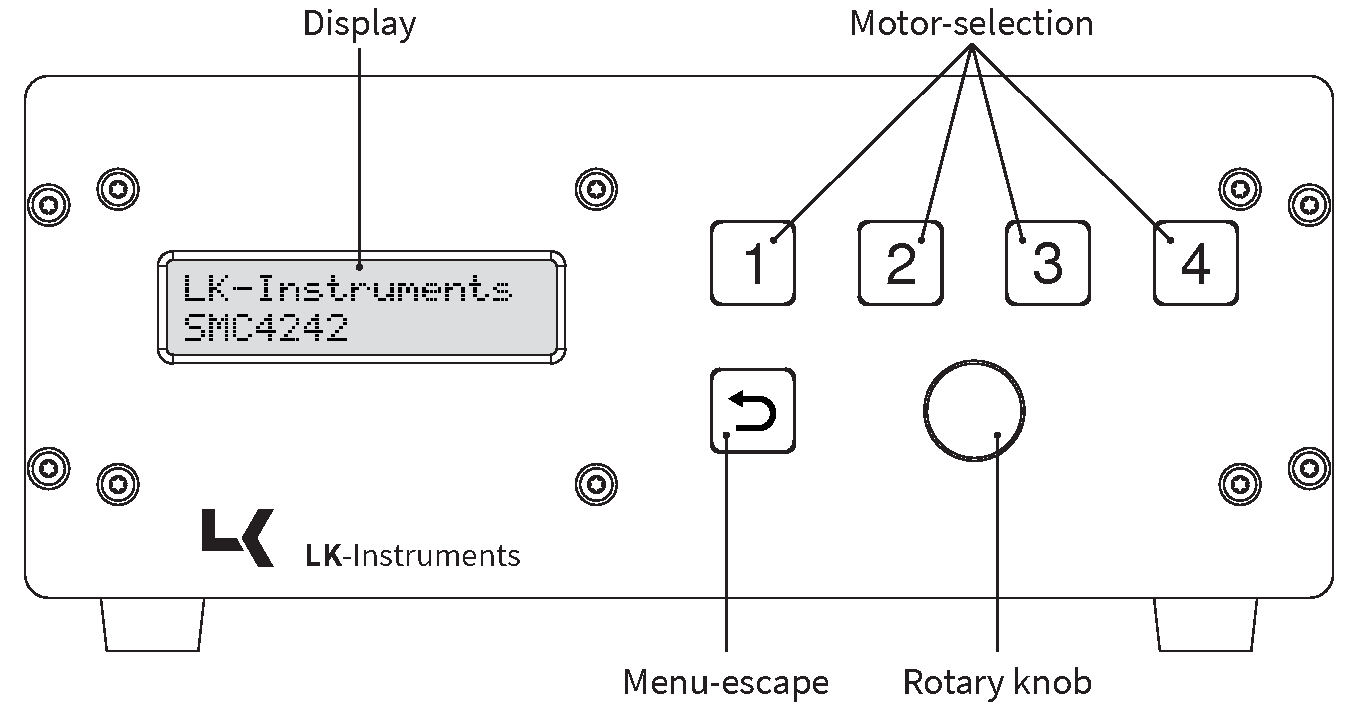
\includegraphics[angle=0,origin=c,width=1\textwidth]{./grafiken/MG22131_front_text_2.pdf}
  \caption[Front view of \productNumber .]{Front view of the \productNumber ~\productName .}
  \label{frontpanel}
\end{figure}

\begin{figure}[h]
  \centering
  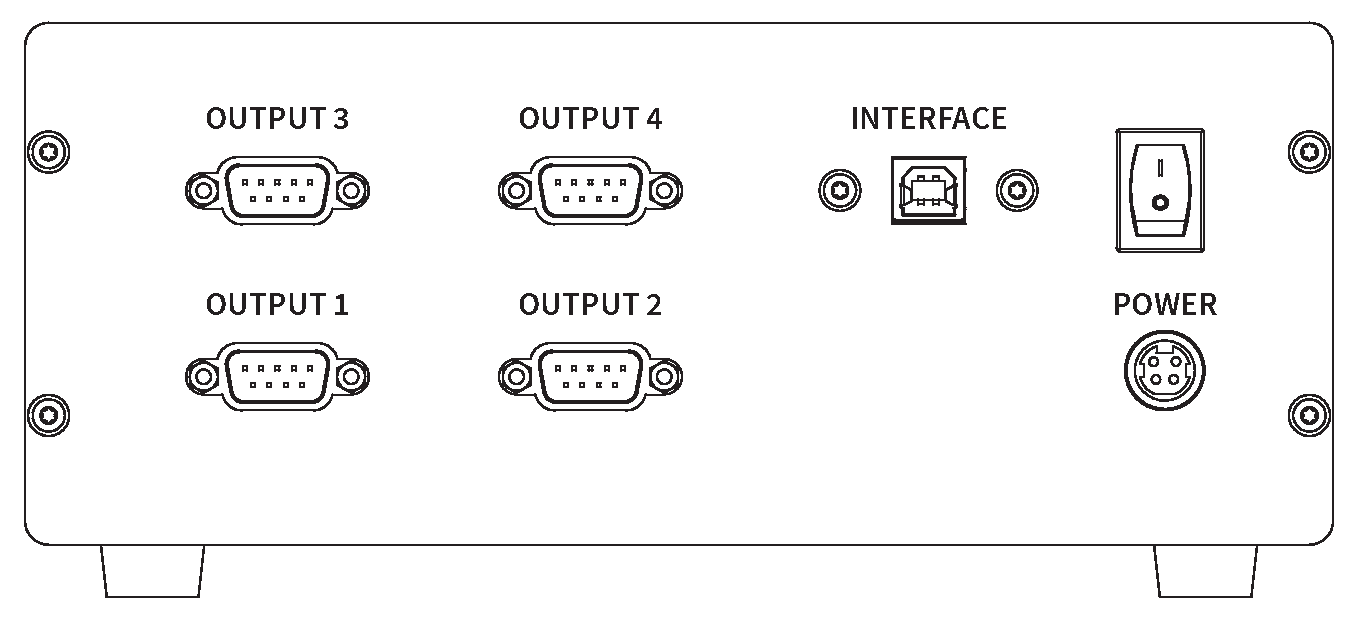
\includegraphics[angle=0,origin=c,width=1\textwidth]{./grafiken/MG22131_back_text.pdf}
  \caption[Rear view of \productNumber .]{Rear view of the \productNumber ~\productName .}
  \label{frontpanel}
\end{figure}



%\newpage